\vspace{1em}
\subsection{Ερώτημα 3-1-3}
Ακολουθούν τα διαγράμματα της ενέργειας αλλά και της μετρικής EDP (Energy Delay Product)
για τα προηγούμενα πειράματα: 
\begin{minipage}{\textwidth}
   \begin{center}
      \fbox{\textlatin{\textbf{\textit{Grain Size: 1}}}}\\
      \vspace{3mm}
      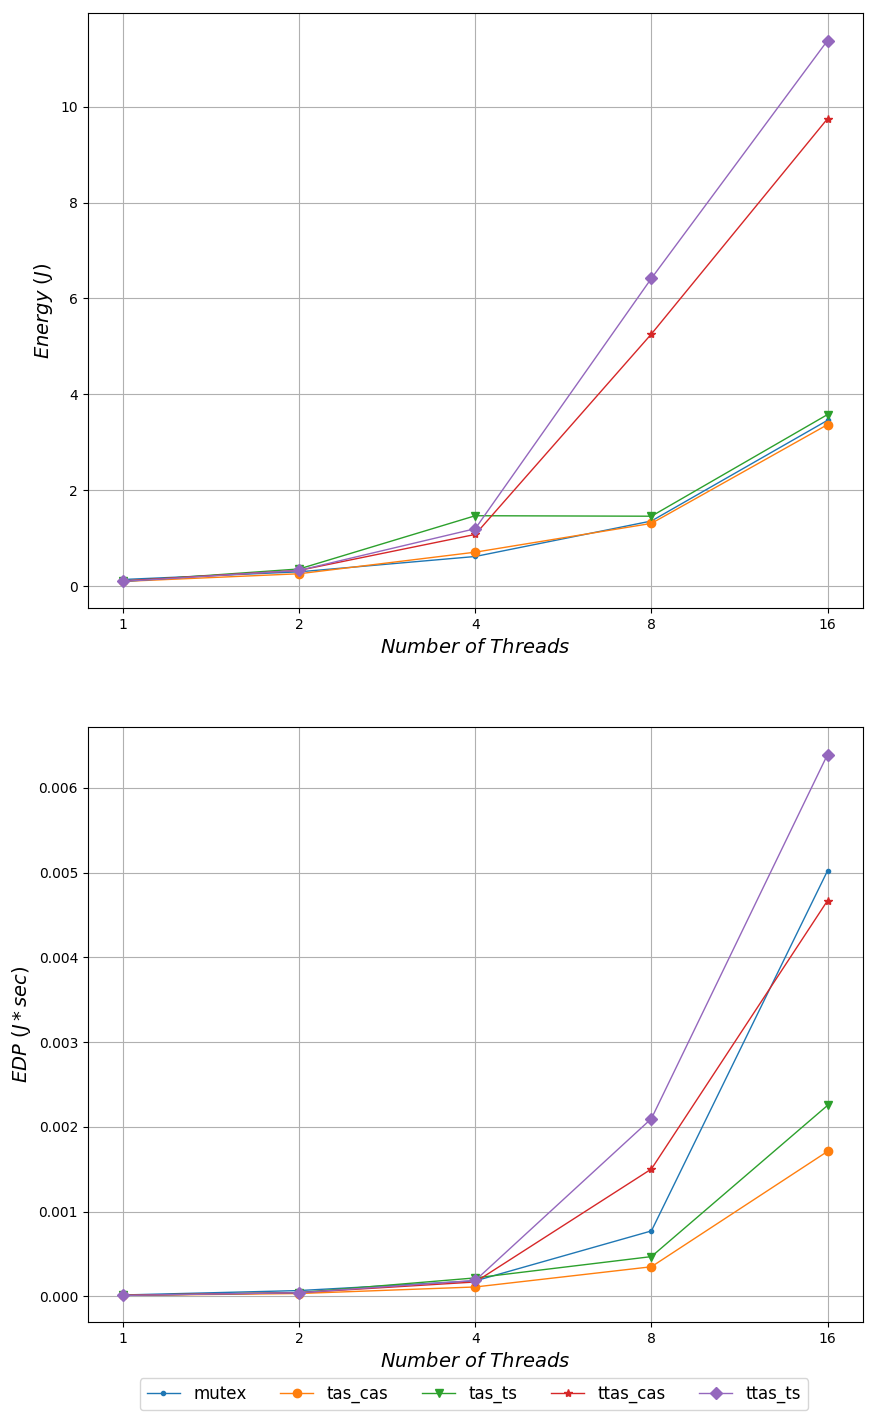
\includegraphics[width=0.7\textwidth]{./graphs/sniper/energy/grain-1.png}
      \vspace{6mm}
   \end{center}
\end{minipage}

\begin{minipage}{\textwidth}
   \begin{center}
      \fbox{\textlatin{\textbf{\textit{Grain Size: 10}}}}\\
      \vspace{3mm}
      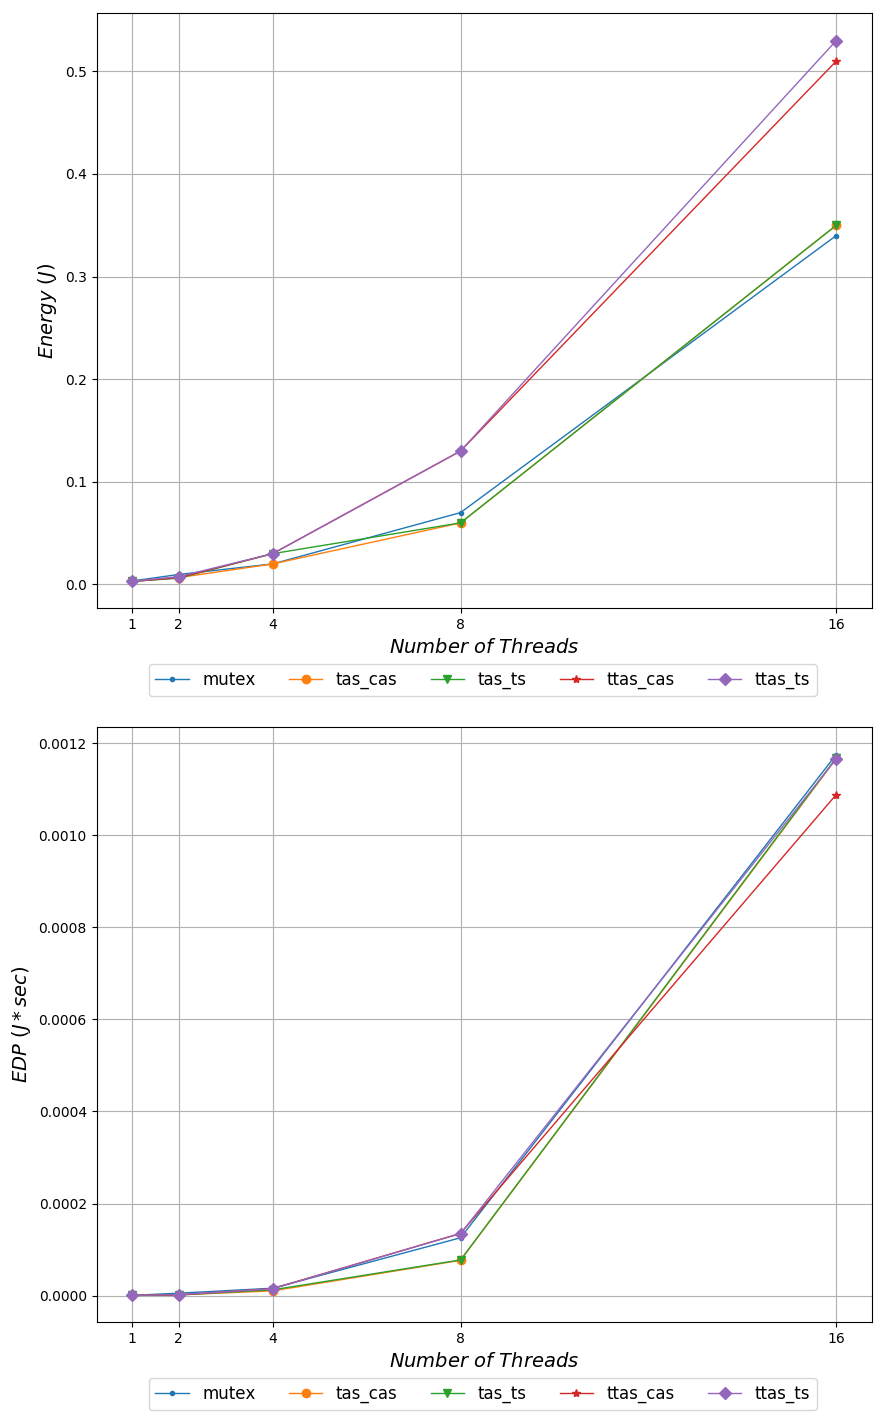
\includegraphics[width=0.7\textwidth]{./graphs/sniper/energy/grain-10.png}
      \vspace{6mm}
   \end{center}
\end{minipage}

\begin{minipage}{\textwidth}
   \begin{center}
      \fbox{\textlatin{\textbf{\textit{Grain Size: 100}}}}\\
      \vspace{3mm}
      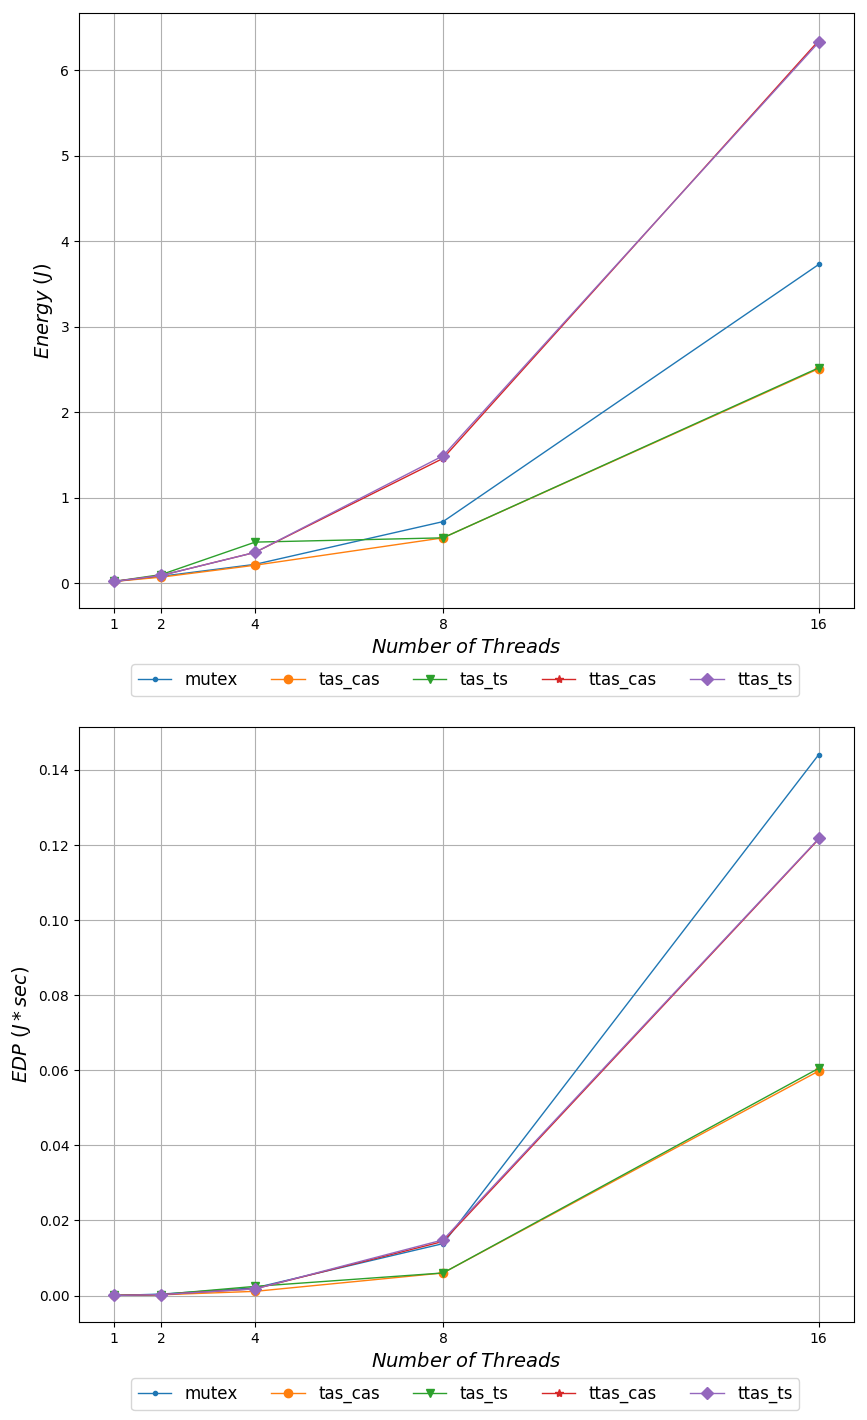
\includegraphics[width=0.7\textwidth]{./graphs/sniper/energy/grain-100.png}
      \vspace{6mm}
   \end{center}
\end{minipage}

\paragraph{Σχόλια - Συμπεράσματα:}
Παρατηρούμε πως η ενέργεια αυξάνεται σχεδόν εκθετικά με το πλήθος των νημάτων.
Ειδικότερα όταν το πλήθος αυτό γίνει από 8 νήματα σε 16 η ενέργεια που καταναλώνεται
είναι σημαντικά μεγάλη. 

Επίσης, βλέπουμε πως για μεγαλύτερα grain size 10 και 100, οι μηχανισμοί
TTAS\_CAS και TTAS\_TS σημειώνουν πολύ υψηλότερη κατανάλωση ενέργειας για μεγάλο
αριθμό νημάτων σε σχέση με τις υπόλοιπες υλοποιήσεις. Αυτό αιτιολογείται από το
γεγονός ότι κάθε νήμα που προσπαθεί να πάρει το κατειλημμένο lock κάνει τοπικά
sniping πάνω στην cache του με συνεχόμενα reads τα οποία κοστίζουν ενεργειακά
πολύ περισσότερο συγκριτικά με τα τα stalls εξαιτίας cache miss ή κατειλημμένο
bus που εμφανίζονται στην περίπτωση των Test-and-set υλοποιήσεων. Σε όλες τις
παραπάνω περιπτώσεις φθηνότερο ενεργειακά φαίνεται να είναι ο μηχανισμός TAS.

Αναφορικά με τη μετρική EDP, αξίζει να σημειώσουμε ότι για grain size 10 οι
καμπύλες τείνουν να ταυτιστούν, και άρα οι μηχανισμοί μπορούν να θεωρηθούν
εξίσου καλοί από πλευρά Energy Delay Product. Στη γενική περίπτωση όμως, με αυτό
το κριτήριο κερδίζουν οι μηχανισμοί TAS-CAS και TAS-TS. Όσον αφορά το μηχανισμό
MUTEX έχει τη χειρότερη επίδοση κρίνοντας με τη μετρική EDP για μεγάλο πλήθος
νημάτων (>8), ανεξαρτήτως grain size.